\section{Results}

This chapter shall discribe, compare and evaluate the results of 3 optimalisation cases. 
\begin{itemize}
	\item Maximum power production
	\item Power production at 80 \% 
	\item Power production at 60 \% 
\end{itemize}
For all these cases was a 9 turbine windfarm used as shown in fig... And were simulated under constant 8 m/s windconditions.

  --
 
 
 \textit{Case 1: maximum power production: }
 This, first, case is used to determine the maximum power output that the 9 turbine farm can extract from the previousely described windconditions, this case neglects the loads.
 

 \textit{Case 2 and 3: Power production at 80 and 60\%: }
 These cases are run at 80 and 60 percent of the maximum power output determinend in the first case. The goal of these cases is to find the optimal running procidure given a required constant poweroutput. the required power output chosen for this paper is linkt to the maximum posible, since ...why? 
 



\begin{figure}
	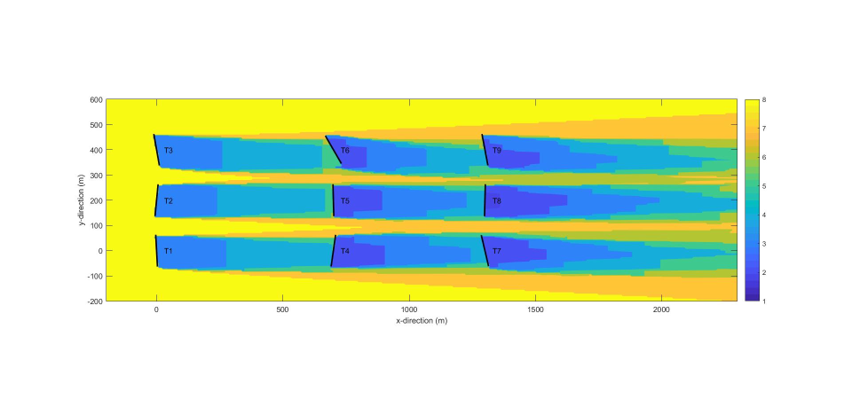
\includegraphics[width=\linewidth]{./Figures/plotje.png}
	\caption{page filler, not the accurate figure.}
	\label{fig:case1turbs}
\end{figure}

	\begin{figure}
	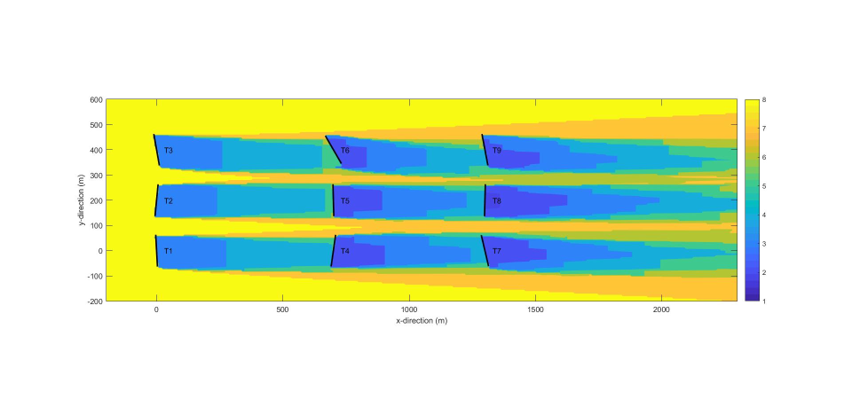
\includegraphics[width=\linewidth]{./Figures/plotje.png}
	\caption{page filler, not the accurate figure.}
	\label{fig:case2turbs}
\end{figure}

 \begin{figure}
 	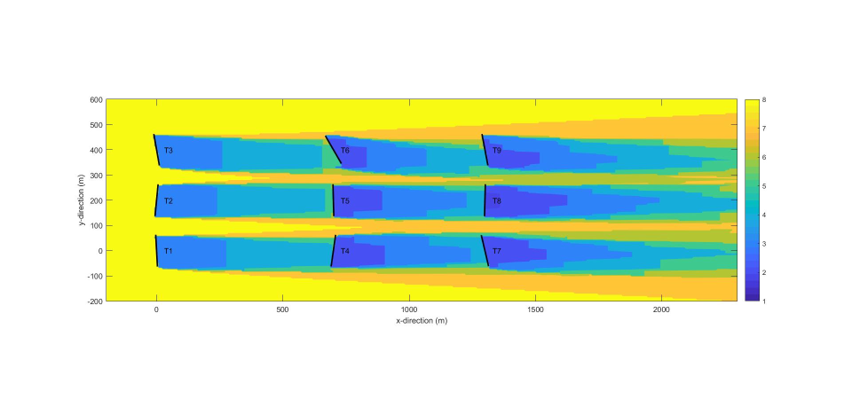
\includegraphics[width=\linewidth]{./Figures/plotje.png}
 	\caption{page filler, not the accurate figure.}
 	\label{fig:case3turbs}
 \end{figure}

\begin{figure}
	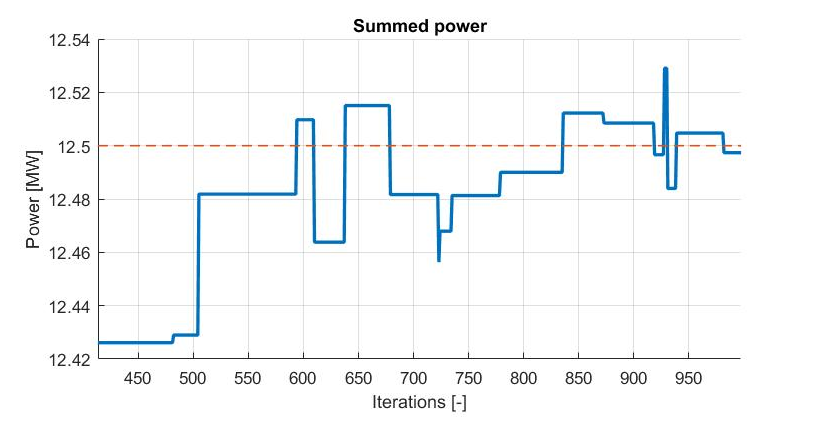
\includegraphics[width=\linewidth]{./Figures/sumpowerexample.png}
	\caption{page filler, not the accurate figure.}
	\label{fig:case1power}
\end{figure}

\begin{figure}
 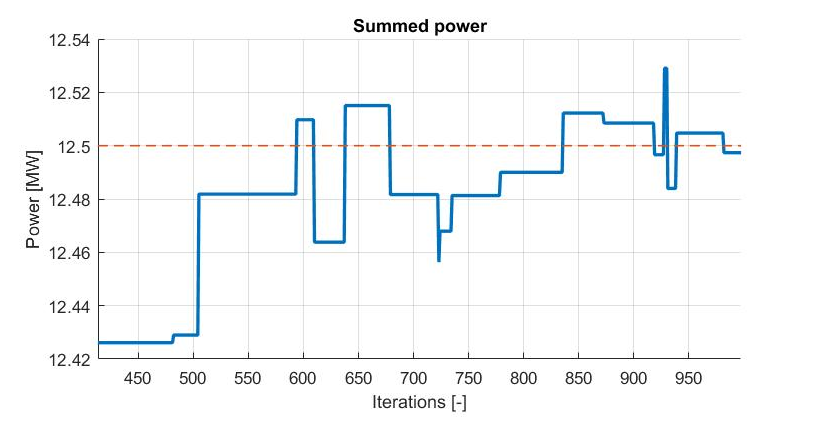
\includegraphics[width=\linewidth]{./Figures/sumpowerexample.png}
 \caption{page filler, not the accurate figure.}
 \label{fig:case2power}
\end{figure}

 \begin{figure}
 	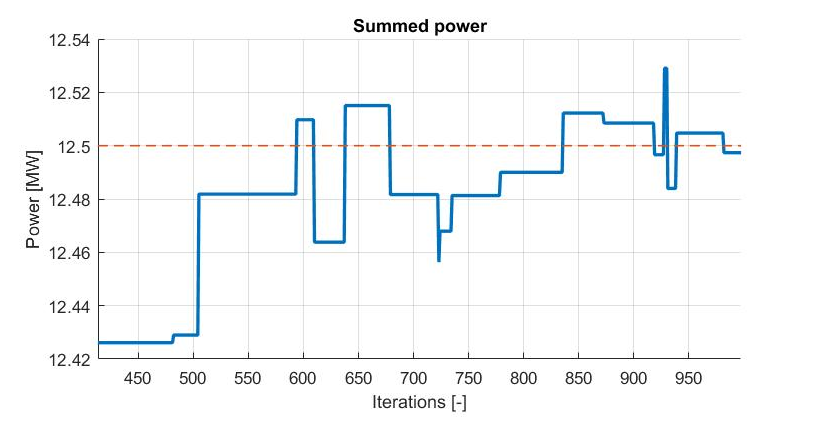
\includegraphics[width=\linewidth]{./Figures/sumpowerexample.png}
 	\caption{page filler, not the accurate figure.}
 	\label{fig:case3power}
 \end{figure}
 
--------------------------------------------------
\subsection{Comparing}


\textit{Power converges}
	reading out the maximum power, stating that power production does indeed aproach the ref power
	
	
\textit{DELs decrese}
	comparing loads, also among eachoter, wat is the effect of lower ref power on the loads/
	
	
\textit{More?}   
 ....

  	
 
----------------------------------------------------   
         